\zzcommand{\heightProfile}{h_{\text{profile}}}
\zzcommand{\heightSubsid}{\height_{\text{subsid}}}
\zzcommand{\heightCoral}{\height_{\text{coral}}}
\zzcommand{\coralMin}{z_\text{coral min}}
\zzcommand{\coralMax}{z_\text{coral max}}

\graphicspath{ {./figures/cGAN_figures/} }

\chapter{Automatic generation of coral reef islands}
\label{chap:coral-island}
\teaser{
	\centering
    \autofitgraphics[]{terrianGAN.png, terrainGAN_result.png}
	% 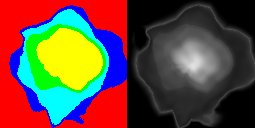
\includegraphics[width=0.6\linewidth]{terrainGAN.png}
	% 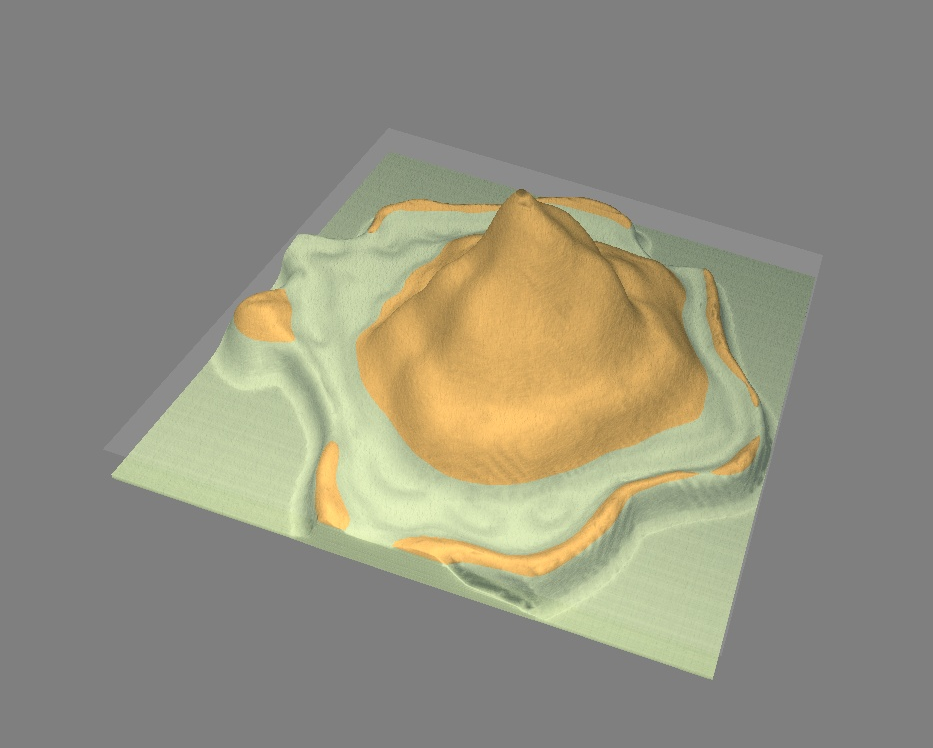
\includegraphics[width=0.3\linewidth]{terrainGAN_result.png}
	\caption{Caption.}
	\label{fig:teaser_cGAN}
}

\abstract 
% In this chapter, we proposed a procedural method for the generation of single circular islands using user sketching from two points of view: a top view and a profile view. These points of view are chosen as they are the most common way to represent describe an island in geological and remote sensing domains. The addition of a user defined wind field completes the assumptions done in this chapter for the generation of islands, more specifically volcanic islands. Given these three inputs, a height field of the island is generated. The inputs can be randomly created, which can lead to the automatic generation of thousands of island models automatically. We will use an out-of-the-box conditional Generative Adverserial Network (cGAN) model, fine tuned on a dataset composed of the many automatic examples on which data augmentation is applied in order to remove constraints from our synthetic island generator, allowing more control to the user on the resulting height fields.
In this chapter, we propose a procedural method for generating single circular volcanic islands using user sketching from two perspectives: a top view, which defines the island's shape (horizontal dimensions), and a profile view, which outlines its elevation and terrain (vertical dimensions). These perspectives, commonly used in geological and remote sensing domains, are complemented by a user-defined wind field, applied as a distortion field to deform the island's shape, mimicking the effects of wind and waves. Based on these inputs, our method generates a height field of the island. This algorithm is capable of creating many different island models, and we have generated thousands of exemplars to compose the dataset used for training a conditional Generative Adversarial Network (cGAN). By applying data augmentation, the cGAN allows for even greater variety in the generated islands, providing users with more control over the shape and structure of the final output.
\pagebreak 

\minitoc

\section{Introduction}
\label{sec:coral-island_introduction}

Coral reef islands emerge from the dynamic interaction between volcanic activity and coral reef growth. These islands begin as volcanic formations, created by magma erupting through the ocean floor and accumulating layers of volcanic rock until the island rises above sea level. These volcanic islands, often characterized by steep, mountainous terrain and a central volcanic peak, provide a foundation for the development of coral reefs in the surrounding warm, shallow waters.

As the volcanic island establishes itself in tropical or subtropical regions, conditions are typically ideal for coral growth. Corals, thriving in clear, warm waters, begin to build extensive reef structures around the island. Initially, this coral growth forms a fringing reef, which is attached directly to the island's shoreline. Over time, as the volcanic island begins to erode and sink (subsidence) the coral reef continues to grow upward to stay in the photic zone, the uppermost layer of the ocean that recieve sunlight. This leads to the formation of a barrier reef, which lies further from the shore, often separated from the island by a lagoon.

In the most advanced stages of this process, the volcanic island may submerge entirely beneath the ocean's surface, leaving behind only the coral reef. This results in the creation of an atoll. The formation of such coral reef islands represents a gradual transition from a prominent volcanic landmass to a coral reef-dominated structure. 

Geologically, the interaction between the sinking volcanic island and the upward growth of the coral reef is a continuous and dynamic process. Over time, the physical appearance of the island may change as erosion and reef growth reshape its form.

% - Definition of coral reef islands \\
% ** Different types of coral reef islands \\
% *** Here, volcanic islands \\
% - Presentation of corals \\
% - Difference from regular landscapes \\
% ** Concept of corals \\
% *** Long-term evolution (island) and short-term evolution (corals) \\
% **** Geological process of island subsidence \\
% - ...

\subsection{Multiple theories}
- Complexity of coral reef ecosystems \\
** Biological diversity \\
*** Varied species of corals and their differing growth patterns \\
*** Interaction with marine flora and fauna \\
** Environmental factors \\
*** Influence of water temperature, salinity, and light availability \\
*** Impact of ocean currents and wave action \\
- Geological processes \\
** Dynamic nature of earth's crust \\
*** Plate tectonics and volcanic activity \\
*** Subsidence and uplift processes \\
** Variations in sea levels \\
*** Historical fluctuations due to glacial and interglacial periods \\
*** Current sea level rise and its impact on coral reefs \\
- Historical and technological context \\
** Historical developments in marine science \\
*** Early exploration and observations by naturalists like Darwin and Wallace \\
*** Advances in geological and oceanographic methods \\
** Technological advancements \\
*** Development of deep-sea exploration tools \\
*** Use of sonar mapping, core sampling, and seismic surveys \\
- Limitations of early theories \\
** Inadequate data and observation \\
*** Limited access to deep-sea environments in the 19th and early 20th centuries \\
*** Reliance on surface observations and anecdotal evidence \\
** Evolving scientific understanding \\
*** Changes in scientific paradigms and theories over time \\
*** Integration of new findings and methodologies \\
- Different perspectives and disciplines \\
** Geological vs. biological perspectives \\
*** Focus on geological processes like subsidence and sea level change \\
*** Emphasis on biological factors such as coral growth and reproduction \\
** Interdisciplinary approaches \\
*** Collaboration between geologists, marine biologists, and oceanographers \\
*** Diverse methodologies leading to different interpretations \\
- Regional and case-specific variations \\
** Geographical differences \\
*** Variations in reef types and formations across different regions \\
*** Influence of local environmental conditions and geological settings \\
** Case studies of specific islands \\
*** Unique formation histories of individual atolls and coral reef islands \\
*** Examples from the Pacific, Indian, and Atlantic Oceans \\
- Ongoing research and discoveries \\
** New findings and theories \\
*** Continuous exploration leading to new hypotheses and models \\
*** Advances in climate science impacting understanding of historical sea levels \\
** Reevaluation of existing theories \\
*** Critical assessment of long-standing theories with new data \\
*** Adaptation and refinement of theories over time

\subsubsection{Theory 1: Subsidence theory}
- Origin and proponents \\
** Charles Darwin (The Structure and Distribution of Coral Reefs, 1842) \\
** Alfred Russel Wallace \\
- Mechanism \\
** Initial formation around a volcanic island (fringing reef) \\
** Gradual sinking of the volcanic island (subsidence) \\
** Transition to a barrier reef with a lagoon \\
** Complete submersion of the volcanic island leading to atoll formation \\
- Supporting evidence \\
** Observations from the HMS Beagle voyage \\
** Modern geological surveys and core samples

\subsubsection{Theory 2: Growth on submarine mountains theory}
- Origin and proponents \\
** John Murray \\
** Alexander Agassiz \\
- Mechanism \\
** Coral colonization on underwater mountains (guyots) \\
** Vertical growth of corals towards the sea surface \\
** Formation of atolls without the need for subsidence \\
- Supporting evidence \\
** Studies on deep-sea coral formations \\
** Distribution of guyots and seamounts in tropical regions

\subsubsection{Theory 3: Sea level change theory}
- Origin and proponents \\
** Reginald Daly (The Coral Reef Problem, 1915) \\
- Mechanism \\
** Impact of glacial and interglacial periods on sea levels \\
** Lowered sea levels exposing coral reefs, allowing vertical growth \\
** Rising sea levels creating conditions for atoll formation \\
- Supporting evidence \\
** Geological records of sea level changes \\
** Correlation with coral reef growth periods

\subsubsection{Theory 4: Erosion and sedimentation theory}
- Origin and proponents \\
** Maurice Ewing \\
** William Donn \\
- Mechanism \\
** Erosion of coral reefs by waves and currents \\
** Accumulation of coral debris forming islands \\
** Continuous process of erosion and sediment deposition \\
- Supporting evidence \\
** Sediment analysis around coral reefs \\
** Observations of island formation from coral rubble

\subsubsection{Theory 5: Platform reef theory}
- Origin and proponents \\
** William Morris Davis \\
- Mechanism \\
** Coral growth on stable continental or insular platforms \\
** Formation of reef structures (platform reefs) \\
** Development into coral reef islands when conditions are favorable \\
- Supporting evidence \\
** Studies on platform reefs and their distribution \\
** Geological stability analysis of coral platforms

\subsubsection{Comparative analysis}
- Similarities and differences \\
** Common themes: coral growth, geological activity, sea level changes \\
** Differences in primary mechanisms (subsidence vs. growth on seamounts) \\
- Complementary aspects \\
** Integration of multiple theories for a comprehensive understanding \\
** Case studies showing multiple processes at work 

\subsubsection{Modern advances and technologies}
- Geological surveys \\
** Core sampling techniques \\
** Seismic and sonar mapping \\
- Environmental studies \\
** Impact of climate change on coral growth and sea levels \\
** Conservation efforts and their implications for island formation

\subsection{Darwinian theory}
- Several theories \\
- Difficulty in studying environments \\
** Use of observations \\
- Theory refuted by \cite{Droxler2021} \\
** But it's too early to judge \\
** Practical for our case. \\
- ...


\subsection{Overview}
- Proposed tool \\
** Sketching the island \\
** Sketching the profile \\
** Wind simulation \\
- Automation of examples \\
** Data augmentation \\
- ...

\section{Related works}
\label{sec:coral-island_related-works}
An intuitive approach for island generation is to use a height field produced through Perlin or Simplex noise functions and apply a falloff map above it. A falloff map is a function $\R^2 \to [0, 1]$ that can be multiplied by the height function to attenuate it, describing a global shape of the island. When using another noise function for the generation of the falloff map, an infinite terrain of islands can be created. This approach, however, does not take into account geological or biological factors, which then make it feel less natural. Control on the noise functions is not intuitive for the user.

Recent works have focused their terrain generation method towards the use of the uplift formulation \cite{Cordonnier2016,Cordonnier2017a,Schott2023,Tzathas2024}. In these models, the user describe areas that are uplifted, which can be seen as areas where heat is produce under the Earth mantel, and the algorithm tries to find an equilibrium between the uplift function and an erosion function. The governing equation for the uplift-erosion, called the stream power equation, is defined as a rate of growth, or increase of height $h$
\begin{align}
    \frac{\partial h}{\partial t} = u - s^n a^m + \Delta h
\end{align}
with $u$ the uplift force and $s^n a^m$ a formulation for fluvial erosion with geomorphological constants $m$ and $n$ with a slope $\Delta h$. the drainage area $a$ represents the area form which all the water pass througha point $\p$. Finding a solution by iteration creates realistic slopes on the sides of heat points, resembling at young mountains. While the initial input, a 2D scalar field representing the uplift force, is a simple user interaction, many manipulations like domain warping can be added to distort the field, resulting in much more varied outputs. Furthermore, the solving process being function of time, the user may feel like interacting during the formation of mountain ranges. However, the resulting landscapes are limited to the scope of mountain ranges.

Other landscape modelisation techniques involve the use of sketching. A sketch is mainly used on a plane, a 2D image, which makes it uneasy to add 2.5D or 3D features in a terrain. Some workaround have been explored to draw using more two points of view \cite{Gain2009} to add more information on the expected output. Another work use the point of view of a player on the ground to add the height information \cite{Tasse2014}. 

** Added radial constraint to simplify interaction \\
- Geological modeling \cite{Patel2021} \\
** For us, it's hard to know what's happening underground (?) \\
- Unlike the literature, integration of the underwater part \\
** Integration of observation data into our process \\
*** -> Typical shape and profile of an island \\
** Difficult to integrate physical simulations due to uncertainty \\
- Layer-based generation could improve the realism of examples by considering layer/environment interactions. \\
- ...


Most recent works, however, leverage the capacity of neural networks for turning a sketch into a 2.5D terrain. \citep{Guerin2017} use conditional Generative Adverserial Networks (cGAN) to encode terrain features as strokes and polygons in images, that are then transformed into an height field as output of the network. In these methods, strokes are rasterized to form a final image, which may lose precision and information. Each terrain feature, like rivers, crests or level sets, are described in a different channel to avoid losing all information after convolutions and pooling layers. 

Networks that take directly parametric curves and polygons are not used as the number of input is generally set in advance, making it limited in its scope.

The original work of cGAN \cite{Isola2017} use a single channel as input, for which each pixel describe an identifier of the element at this position [A REDIRE]. In out method we use this technique to let the user modify the content of its terrain more easily as it does not require any different software for the input image editing. The problem of the one-pixel wide features vanishing is avoided by representing only regions.

In order for neural networks to be trained, a large amount of data have to be available. Coral reef islands representing a very small portion of  Earth's surface. In this work we decided to generate the data ourselves in order to train a network. 

\section{Example generation}
\label{sec:coral-island_example-generation}
Generating synthetic data for the training of a neural network introduce a bias in the dataset. We use observations from old and recent expeditions in order to define in advance the biases that are being introduced. First, we will take advantage of the different characteristics that are commonly found in coral reef island. The assumptions we will use are listed below:
\begin{enumerate}
    \Item{} Islands have a relatively round shape: the heat under Earth's mantel comes usually from a single point, making the uplifting force of volcanic islands radial around the epicenter. Plus, see erosion has the effect of smoothering corners.
    \Item{} Coral grows to a constant height around the island: coral polyps have to have access to sunlight to survive, resulting in a band of living corals starting from the water level to a certain depth of about 30m where coral colonies become much scarcer. 
    \Item{} All features are radial: the main features we want to create , that are island, beaches, lagoon and coral reef, are always in this order and are highly correlated to the shape of the island. We can place the assumption that the interface between each of these regions are radial around the island center.
    \Item{} Islands deformations are caused by winds and waves: the main natural phenomenon that morph an island into a shape is the effect of aerial and coastal erosion on its borders. We can leverage this idea by using a wind velocity field to apply domain wraping for the final height field. This operation allows the result to have non-radial and concave regions, removing the limitations listed above.
    \Item{} Islands are independent of each other: an island has no notable influence on another's elevation characteristics. We can then consider having multiple islands created with an algorithm and translated next to each other without finding notable incoherencies as long as the islands are not overlapping.
    \Item{} The profile is relatively identical all around the island: resulting from the point 3, as the regions of interest are in consecutive order, the profile in any direction of the island have similar shape, except for their scale.
    \Item{} The subsidence only affects the ground, but not the coral reefs.
\end{enumerate}

These assumptions are not completely exact, but provide a simplified model of the coral formation following Darwin's theory.

In this work we created an editor that allows to manipulate radial curves, allowing a user to layout the top view of the island, but also the side view.

% - We use Darwin's theory in our case because generation is relatively simple. \\
% - 2 steps: \\
% ** Generation of the island \\
% ** Generation of the reef \\
% - Numerous assumptions: \\
% - ...

\subsubsection{Input}
Our method takes as input a top-view sketch and a profile sketch. From these two sketches we can apply a revolution to model in 3D the shape of the island. A wind map, a 2D vector field, is used to simulate erosion through warping. Finally, information about the water level and a subsidence rate is provided to simulate the the sinking of the island and the growth of the coral reef.

In this initial algorithm, the island is centered in the scene. The different regions that compose the landscapes are defined by polygons whose vertices are defined in polar coordinates $(\radius, \angl)$ with $\radius \geq 0$, constraining each region to contain the center of the island. 

The different regions we consider are mountains, island borders, beaches, lagoon, reef crests and abyss limits [ADD FIGURE]. We define in advance an order in which these regions appear, from the center of the island to the open ocean. This limits the radius of a region to be lower or equal to its successor's radius: $\radius_{i-1}(\angl) \leq \radius_{i}(\angl)$. 

The profile of the island is given as a 1D function $\heightProfile: [0, 1] \to \R$. The height at the center of the island is defined as $\heightProfile(0)$, and each region $i$'s limit is defined at $\heightProfile(t_i)$ with $t_i = \frac{i}{n - 1}$. We can then use a linear interpolation to determine the height $h(\p) = \heightProfile(t_{\p})$ at any point $\p$ inside a region. Using the polar coordinates of $\p = (\radius_{\p}, \angl_{\p})$, we find $t_\p = \lerp \left( t_{i-1}, t_i, 1 - \frac{\radius_{\p} - \radius_{i-1}}{\radius_i - \radius_{i-1}} \right)$.

The user can remove the radial constraint using a third interaction process, a deformation field $\warp: \R^2 \to \R^2$ simulating the effect of wind and waves on the island. We can then compute the final height $h(\warp \circ \p) = \heightProfile(t_{\p})$, or, as the implicit modeling community would write it, $\Tilde{h}(\p) = \warp^{-1} \circ h$.

While we did not study it in depth, one can add a resistance function $\rho: [0, 1] \to [0, 1]$ defined in the same manner as the profile function $\heightProfile$ which can be seen as an attenuation of the deformation field $\Tilde{\warp} = \rho(t_{\p}) \warp$. We keep the same formulation $\Tilde{h}(\p) = \Tilde{\warp}^{-1} \circ h$.

Once the initial terrain surface is computed, the algorithm apply the simulation step with the water level and subsidence rate provided.

% - Sketching of the island from above + profile view \\
% - Wind strength \\
% - Water level \\
% - Subsidence rate \\
% - ...

\subsubsection{"Simulation"}

The simulation step for the coral reef generation is not physically based, but based on observation.

We know that the coral reefs starts their formation at the borders of the island, close to the water surface and down to around 30m, and, while the ground is subsiding, it can remain close to the water surface when it "keeps up" (continues growing while the water level changes). 

In our simulation, we use the initial height field $\height_0$, but also the same height field after subsidence occured. We will consider the effect of subsidence as a scale in the Z-direction for all the points in the original height field $\heightSubsid = (1 - \lambda) \height_0$ with $\lambda$ the subsidence state given by the user.

The lifespan of volcanic islands being multiple orders of magnitude higher than coral reefs (multiple millions of years against about ten thousands years), we will neglect ground surface geomorphing during the reef simulation. 

Let's investigate on the common shape of a coral reef. From the open sea to the island borders, we have the fore reef zone, the reef crest, and the reef flat zone. We focus our reef model around the crest as it remains close to the water level. Behind it, we find a small slope then a lagoon (respectively the back reef and lagoon zone, composing the reef flat zone) and in front of the reef, a stronger slope then a wall (respectively the buttress zone and the deep fore reef, composing the fore reef zone). We will model each of these parts individually, then blend them with the initial height field.

We can place all these limits in the field with:
\begin{Itemize}
    \Item{} Crest min are at $\height_0 = \coralMax$,
    \Item{} Crest max are at $\height_0 = \coralMin$,
    \Item{} Lagoon min are at current island borders $\heightSubsid = \Wlevel$,
    \Item{} Lagoon max are at Crest min - back reef width,
    \Item{} Deep fore reef min at Crest max + buttress width,
    \Item{} Deep fore reef max at Crest max + buttress width + fore reef width
\end{Itemize}

Fixing a depth for the lagoon, reef crest, buttress end and abysses, we now have constraint heights that partially cover the terrain. We connect the missing parts using the cubic rational smoothstep function $\smooth(t) = \frac{x^3}{3x^3 - 3x + 1}$ proposed by Inigo Quilez.

We then have a height field $\heightCoral$ for the coral landscape. We can blend the island and the coral height fields using a smooth max function, derived from the smooth min functions also proposed by Quilez: $\max(a, b) = b + k \left( \frac{\frac{\left( a-b \right)}{k}}{1-2^{\frac{\left( b - a  \right)}{k}}} \right)$ with $k$ a tolerence value. 


While the results may not be physically accurate at all, we allow the user for much more control on the output.

One can modify the filling by defining a height and slope constraint at each limit as proposed in \citep{Guerin2022}.

% - Subsidence calculated by simple scaling \\
% ** Note: No geological consistency \\
% *** Here, using a zero level to scale in Z \\
% *** No consideration of different soil materials \\
% - Reef growth \\
% ** Does not consider any weather events \\
% ** Considers the "keep up" strategy (as opposed to "give up" and "catch up") [large simplification] \\
% - Wind deformation \\
% ** using directly $f(\p) = f(\warp(\p))$. \\
% - ...

\subsubsection{Output}
We obtain as output a height field of a simplified coral reef island. The main importance of this method is to conserve the semantic of the terrain, as we can always know the location of the island, lagoons, reefs, etc. Keeping track of the semantic has multiple advantages:
\begin{Itemize}
    \Item{} Texturing the surface with respect to the terrain features is easily done.
    \Item{} Terrain augmentation is eased as we can add multiple post-processing methods like the creation of passes, the addition of spurs and grooves patterns, etc.
    \Item{} Subsurface ground material is available, even while working on 2D height fields.
\end{Itemize}
% - Height map of the island's surface \\
% - Island zones and coral zones \\
% - Possibility to recalculate ground height and coral height \\
% - ...

% \subsection{Closed form of coral growth}
% - Proposes a closed-form solution for surface calculation \\
% - Calculation of ground height: \\
% ** Calculation of height by revolution around the origin point \\
% ** Deformation of the revolution profile using the top-down sketch \\
% ** Deformation of the height field by the wind map. \\
% - Calculation of growth: \\
% ** On the initial heightmap, \\
% *** Any surface $z_{min} < h(p) < z_{max}$ becomes coral \\
% *** Calculation of the "low" contour $h(p) = z_{min}$ and "high" contour $h(p) = z_{max}$ \\
% *** ... \\
% - Deformation of the map using the wind map: \\
% ** ... \\
% - ...

\subsection{Labeling of the map}
The feature map paints the pixels corresponding to each of the regions instead of only containing the demarkation lines. Multiple reasons leads to this decision :
\begin{Itemize}
    \Item{} In the case of two demarkation lines too close to each other, an overlapping can appear at pixel scale, leading to the loss of information of the undelying line.
    \Item{} While this problem is often resolved by using as input an image with $n$ channels, with each of the channel being a binary map of the $n$-th feature. This decision results in needing to modify the cGAN architecture, inducing the need for a full training of the new model as it may not be compatible with an available pretrained model.
\end{Itemize}

In order to label the map, we first rasterize the map using polar coordinates and the 1D functions that represents each features border. 
With the center of the island at the coordinates $(0, 0)$, we get the polar coordinates for any point $(x, y)$ as $\radius = \sqrt{x^2 + y^2}$ and $\angl = \arctan2 (y, x)$. We can then use the label $l \in \N$ with $l = \arg \min_i \left( \radius \leq \radius_{i}(\angl) \right)$. This operation is very fast and completely parallelizable.

We did not include the limits specific to the coral reef previously cited (crest, lagoon, forereef, ...). The reason behind this being that, when a neural network will be trained on this task in order for the generation of the height field directly from a labelled map, we do not want the user to have to consider a large amount of labels.

Once rasterized, the map is warped using the same displacement map $\Tilde{\warp}$ used for the height field deformation. As such, the feature map is directly associated to the height map.

% - Using top-down sketch: \\
% ** Features "Mountain", "Island borders", "Beach" are radial $(\angl, r)$, so we can label each point of the map as the "next" feature \\
% - Using coral simulation information: \\
% ** Provides the labels "Lagoon" and "Reef \{begin, peak, end\}". \\
% - The height map is directly associated to the feature map \\
% - This is perfect to feed a cGAN. \\
% - ... 

\subsection{Automation}
- Take advantage of the radial nature of the features \\
- Some features can be optional (mountains) \\
- Deformation of the feature lines \\ 
** Influence on the radius: $\Tilde \radius(\angl) = \radius(\angl) + \noise(\angl)$ with $\noise$ continuous noise function $2\pi$-periodic. \\
- ...

\section{cGAN}
\label{sec:coral-island_cGAN}
- Conditional GAN: a type of Generative Adversarial Network (GAN) where the generation process is conditioned on additional information. \\
- ...

\subsection{Definition of cGAN}
- Two networks: consists of two neural networks, a generator and a discriminator, which compete against each other. \\
** Generator: takes both random noise and additional information (like class labels or data) to produce synthetic data. \\
** Discriminator: evaluates whether a given data instance is real (from the actual dataset) or fake (produced by the generator), while also considering the additional information. \\
** Additional information: this can be labels, data from other modalities, or any other contextual information that guides the generation process. \\
- Training process: the generator tries to create realistic data to fool the discriminator, while the discriminator tries to correctly classify data as real or fake based on both the data and additional information. \\
- Objective: the goal is to improve the generator's ability to produce realistic data that matches the given conditions and to enhance the discriminator's ability to distinguish between real and fake data. \\
- Applications: used in various domains including image-to-image translation, text-to-image synthesis, and other tasks where generating data based on specific conditions is required. \\
- ...

\subsection{Why cGAN?}
- Flexibility of input \\
- Moving beyond the "radial" input condition \\
- Output even for "inconsistent" data (e.g., ocean in an island) \\
- No math, geometry, geology, or complicated things to master (hehe) \\
- ... 

\subsection{Training}
- ...

\subsubsection{Use of synthetic data}
+ Problem with synthetic data \\
- ...

\subsubsection{Data augmentation}
- ...

\subsection{Model usage}
- ...

\subsubsection{Generation from sketch}
- ...

\subsubsection{Interactive times}
- ...

\subsubsection{Realism}
- ...
